\documentclass{report}
\usepackage{mathtools}
\usepackage{amsmath}
\usepackage{amssymb}
\usepackage{amsfonts}
\usepackage{graphicx}
\usepackage{float}
\usepackage{multirow}
\usepackage{verbatim}

\linespread{1.3}
\setlength{\parindent}{0em}
\setlength{\parskip}{1em}
\setcounter{secnumdepth}{0}
\setcounter{MaxMatrixCols}{20}
\renewcommand{\arraystretch}{1.5}

\newcommand{\ts}{\textsuperscript}
\newcommand{\diff}{\mathop{}\!\mathrm{d}}
\newcommand{\prob}{\mathbb{P}}
\newcommand{\expect}{\mathbb{E}}
\newcommand{\var}{\text{Var}}

\DeclarePairedDelimiter{\abs}{\lvert}{\rvert}
\DeclarePairedDelimiter\norm{\lVert}{\rVert}
\DeclarePairedDelimiter\p{\lparan}{\rparan}

\title{COMS3000 notes}
\author{Joshua Hwang (44302650)}

\begin{document}
\maketitle
\tableofcontents
\chapter*{Prerequisite maths}
We must recall how to calculate the extended Euler's algorithm and discrete
logarithms.

Should be noted for the discrete logarithm to exist,
\begin{align*}
    \log_a (c) \mod n \\
\end{align*}

$n$ must be prime and $a$ needs to be a generator.

I will assume you know how to calculate the extended Euler's algorithm.

\chapter{Information security}
\section{Basic terms}
This first chapter will talk about definitions.

There are three things we can do with risk; accept it, transfer it (insurance)
or reduce it (control it).

Information security is all about protective measures and dealing with potential
damages. Some of these protective measures include; prevantative measures,
detective measures (to know when, how and who caused damage) and reactive
measures (allows us to recover from damages).

The information security can be categorised into the CIA triad.
\begin{description}
    \item [Confidentiality] Prevent unauthorised disclosure of information
    \item [Integrity] Prevent unauthorised modification of information
    \item [Availability] Prevent unauthorised witholding of information i.e. DoS
\end{description}

We can extend these first three aspects with two more
\begin{description}
    \item [Authenticity] Make sure the author/sender is as claimed
    \item [Non-repudiation] People can't escape contracts by claiming that it
        was a forgery.
\end{description}

Being trusted and trustworthy are two separate ideas.
Hopefully the difference is obvious.
Direct trust can be developed by two parties.
Indirect trust involves trusting a third party who claims others are trustworthy.
Trust will be explored later on.

\section{Risk management}
Risk management is the process concerned with identification, measurements,
controls and minimisation of security risks in information systems to a level
appropriate to what the asset is worth.

The following definitions are quite dry and dense so be prepared.

Risk management helps determine and optimise for the appropriate cost/benefit
for protective measures.

Identify, measure, control and minimise or eliminate attacks.
This is done through: risk assessment, cost benefit analysis, selection,
implementation and evaluation of security features and countermeasures and
an overall security review.

The definition of risk as determined by ISO/IEC 27000:2018 is,
`\textbf{effect of uncertainty of objectives}'.
Where an objective is a result to be achieved. (e.g\. our data gets locked up)

The definition of threat as determined by ISO/IEC 27000:2018 is,
`\textbf{potential cause of an unwanted incident,
which can result in harm to a system
or organization}' (i.e. the potential cause of why all our data is held hostage.
Someone gained acces to our system through a phising attack)
Should be noted that hackers and careless employees are threat actors and not
threats.

The definition of vulnerability as determined by ISO/IEC 27000:2018 is,
`\textbf{weakness of an asset or control that can be exploited by one or more
threats}' (e.g.\ work place emails are exposed to the internet which allowed
the attacker
to send the phising attack in the first place)

SQL Injection is a vulnerability.
Sensitive data theft is one of the biggest threats that SQL injection enables.

Buffer overflows is a vulnerability.
Remote code execution is a threat.

The definition of risk assessment as determined by ISO/IEC 27000:2018 is,
`\textbf{overall process of risk identification, risk analysis and risk
evaluation}`.

\section{Risk analysis}
A qunatitative risk analysis largely resolves around the following.
A model for quantifying the cost is taking the expected value of the
event occuring $prob \times impact$.

\begin{description}
    \item [ARO (Annualised Rate of Occurrence)] Number of times a year.

    \item [SLE (Single Loss Expectancy)]
        The impact of a single type of this event occurring.

    \item [ALE (Annualised Loss Expectancy)]
\end{description}

The equation is simple and is as follows,
\begin{align*}
    ALE &= ARO \times SLE
\end{align*}

It is often difficult however to get these probabilities and also to
quantify the impact and cost of an event.

Instead we might use a more qualitative method.
Risk assessment matrices.

\begin{figure}[h]
    \centering
    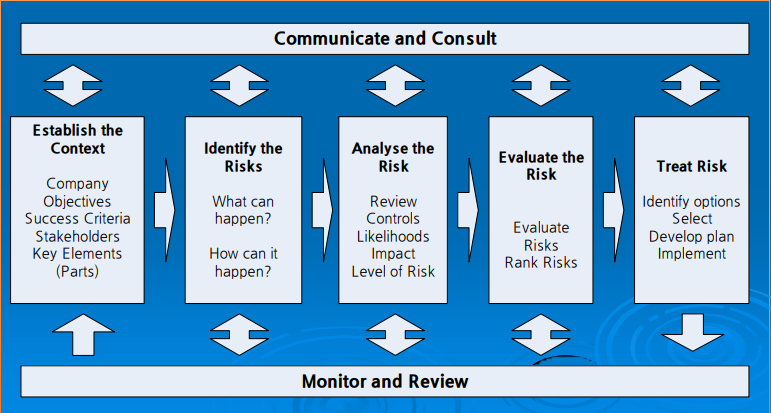
\includegraphics[width=\textwidth]{images/standards-flow.png}
    \caption{ISO31000:2018 Risk Management Principles and Guidelines}
\end{figure}

\chapter{Access Control}
There are two separate but important functions to establish identity:
\begin{description}
    \item [Identification] Determine who the entity is
    \item [Authentication] Verity and prove you are who you say you are.
\end{description}

Authorisation, once identity is established a decision can be made about
granting or denying access.

Most access control is determined by identity. Which has a second benefit of
accountability (we can track who did what when in the system).

\section{Passwords}
Passwords have been the goto for years. It is based on `something you know'.
There are many of problems incluing; forgetting the password, same password for
multiple places, weak passwords, passwords not kept in secret and not changing
default passwords.

Carna botnet was an attempt to scan and attempt default passwords on anything
connected to the internet. It obtained $\approx 500,000$
devices through Telnet mostly embedded systems in 2012.

Passwords can be guessed via bruteforce, socially engineered and tricked out of
humans, eavesdropped and keylogged. Many also store passwords in various places
like password managers which increases risk.

Dictionary attacks and brute-force attacks are known as off-line attacks. This
is where the attacker has access to the hashed passwords (and plenty of time
with them). This is kinda like a ciphertext only attack.

An on-line password attack involves the attacker talking to a live system. This
is obviously much harder since the system might give you timeouts. A clear
example of this is ATMs. Though the password is only 4 digits the ATM `eats' the
card if there are three failed attempts.

Consider the /etc/passwd
which contain the hashed passwords of all users.
What if two users happen to choose the same password?  If a user shares the same
password with another user then they will know the other user's password.

This is solved via SALTing. Unix uses 12 random bits in a modified DES algorithm
to fix this.

\subsection{Authentication with passwords}
How on earth do you send your password over the internet to verify?
You COULD send the hashed password over the network but an eavesdropper can
perform a replay attack.

Instead we choose a Challenge-Response Protocol.
The server gives a client a `challenge', $c$
(often called the nonce, number-used-once)

Client calculates a response which is a cryptographic hash of $c$
and the password
either as $r = h(c||p)$ (concatenation) or $r = h(c XOR p)$.

Note manually choosing the challenge does not affect the strength. The only
requirement is that the challenge only happens once.

\section{Mutli-factor authentication}
Two-factor authentication involves using one of the two methods:
\begin{itemize}
    \item something you know and something you are (password and fingerprint)
    \item something you know and something you have (password and physical key)
    \item something you are and something you have
        (fingerprint and physical key)
\end{itemize}

For example using an ATM requires a card and knowing the PIN\@.

SecureID is a way to have a `physical key' for internet usage. This makes use of
a piece of hardware that generates pseudorandom numbers which are synced with an
authentication server.

\section{Complete Aside}
The idea of using rwsr-xrwx (where s is the SUID or set user id feature) is
called the access control list. An access control list has users (subjects)
and groups which have permissions to do certain operations (access operations)
on certain objects.

\section{Biometrics}
Criteria for good biometrics involve:
\begin{itemize}
    \item Universality (everyone must have one)
    \item Distinctiveness (should be unique for each person)
    \item Permanence (must not change)
    \item Performance (must be fast to recognise)
    \item Acceptability (are people okay using this body part for identification)
    \item Circumvention (how easy to trick the system and perform replay attacks)
\end{itemize}

Tiny fingerprint features called Minutiae are stored instead of an image.

Verification mode is a one-to-one match with a single template in the database.
Identification mode is a one-to-many match.

Intuitively the identification mode is more likely to pop up a false accept.

There are two main types of errors:

False accept (False Match) which allows non-users access thinking they are the
template.

False reject (False Non-Match) which prevents true users from accessing their
own template.

In addition:
Failure to Enrol (FTE) failure to create a valid template from a new user's
input.

I'm trusting that you can actually calculate the false match and false non-match.

\chapter{Cryptography}
\begin{description}
    \item [Cryptography] is about keeping messages secure. It literally means
secret writing.

    \item [Cyrptanalysis] is the science of breaking message security.

    \item [Cryptology] is the theory associated with
        cryptography and cryptanalysis.
\end{description}

The aim of cryptography is confidentiality but it can also be used to
authenticate a user, ensure no messages have been modified and
might even be used for digital signing.

\section{Types of attacks}
Much like in MATH3302 we have the different types of cipher attacks:
\begin{description}
    \item [Ciphertext only]
        The attacker has obtained a piece of ciphertext but no decoding
    \item [Known-plaintext attack]
        The attacker has obtained a piece of ciphertext and its corresponding
        plaintext
    \item [Chosen-plaintext attack]
        The attacker has temporary access to the encryption machine
    \item [Adaptive Chosen-Plaintext attack]
        The attacker has the encryption machine for quite some time
\end{description}

\textbf{Side Channel Attacks} are attacks against an implementation rather than
the algorithm itself. We gain new information like, timing, power consumption
etc.

\section{Hash functions}
Hash functions compress an arbitrarily long input $x$ into a fixed size output.
They should be designed to be easy to compute.

One-way hash functions have the one-way property. It is computationally
infeasable to find $x$ given $h(x)$.
One-way is also called \textbf{pre-image resistance}.

Now cryptographic one-way functions have another property called
\textbf{collision resistance}.

An ideal one-way cryptographic function can be visualised as such.
`Has this input arrived before?' If yes re-return the output. If no, then
make a random sequence for this new input.
This model is called a \textbf{random oracle model}.

\textbf{Strong collision resistance} means its hard to find two distinct
$x_1$ and $x_2$ such that $h(x_1) = h(x_2)$
\textbf{Weak collision resistance (aka 2nd pre-image resistance)}
given a specific
$y=h(x_1)$ it is hard to find $x_2$ such that $h(x_1) = h(x_2)$

To find a weak collision we need $2^n$ but for a strong collision we just need
$2^{n/2}$ since birthday paradox.

A cryptographic hash is considered broken if collisions can be found with
significantly less work than brute force.

An offline attack on passwords is when the attacker has access to the hashes
of the password. The hacker can then apply numerous exploits on the file
to get a collision/reverse the hash.

\section{Cryptography keys}
The problem with using a different and hidden protocol for all communications
between people is that no one can talk to new people. Instead we have
cryptography keys which alter the algorithm in a way that still ensures it's
impractical to crack. This is \textbf{Kerckhoff's Principle},
`\textit{The security of a cipher should rely on the secrecy of the key only.}'

Computational security is measured by, the resources and time necessary for the
attacker to crack the cipher (with the key length we're using)
vs how long the information needs to be kept
secret.

\chapter{Types of ciphers}
As we learnt in MATH3302 there is no way yet to practically measure the security
of a cipher. It's either `too hard' to wrap our heads around or it's founded on
a computational problem that does not have efficient algorithms (yet).
Thus the goal of creating a cipher is computation security,
this is where the best
attack option is brute-force; there are no shortcuts to get to the key.
From here it's purely key length that determines security; it's a simple brute
force job.
The only way we can `prove' this is to show that our cipher is secure against
all currently known attacks.

\section{Old ciphers}
You should have seen and remembered many of these ciphers from MATH3302.

Caeser cipher where each letter is offset by a constant amount (this shift is
the key).

Monoalphabetic substitution cipher where the alphabet is shuffled randomly.

Vigenère cipher is an extension of the Caesar cipher where a secret set of
offsets (usually a word) is periodically used on the plaintext.

One time pads where we extend the Vigenère cipher so the secret word is the
length of the message. The secrete key doesn't get repeated. One time pads
are perfectly secure.

Transposition cipher where we create a matrix of the message (secret rows and
columns) we then read off the matrix in the transpose way.
\begin{figure}[h]
    \centering
    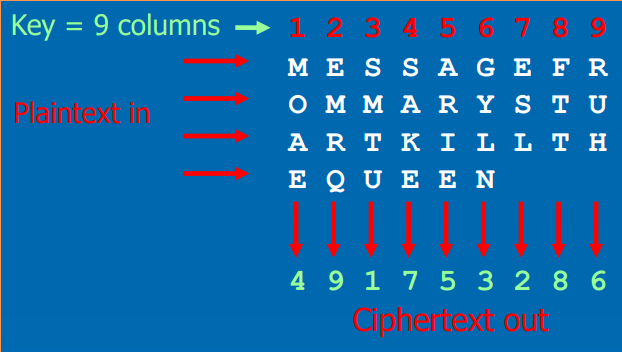
\includegraphics[width=\textwidth]{images/transpositioncipher.png}
\end{figure}

\section{Symmetric ciphers}
Many modern ciphers are product ciphers.
A product cipher is a composition of either substitutions or permutations
(which are also just substitutions). They are iterated several times to increase
security.

Feistel ciphers are what you've already seen in MATH3302 so I hope you remember
them. Many product ciphers are Feistel ciphers.

Transposition involving swapping the two blocks being encrypted.
Substitution using S-boxes.
Decryption is also encryption but with the round keys in reverse order.

Note that the F function does not have to be reversible since XOR twice results
in the original solution.

\subsection{Block ciphers}
\subsubsection{DES}
DES uses 16 rounds with 64 bit blocks and 56-bit key with 8 bits for parity.
The round function expands 32 bits into 48 bits.
The S-box converts 6 bits into 4 bits

The DES challenge was an attempt to break the DES by bruteforce.
\begin{description}
    \item [1997] took 3 months
    \item [1998] took 3 days and cost \$250K
    \item [1999] took 22 hours with machine created from the 1997 and 1998 challenges
    \item [2006] took 7 days for \$10K (COPACOBANA)
\end{description}

Each new key bit doubles the time required for a brute force. This means a
128-bit key will take 90 billion billion years for COPACOBANA to crack it.

Choosing to double DES via
\begin{align*}
    c &= E_{K2}(E_{K1}(p)) \\
    p &= D_{K1}(D_{K2}(c))
\end{align*}

Now we should theoretically have double the key size. Unfortunately 2-DES is
vulnerable to meet-in-the-middle attacks.

If you manage to find the inbetween value (so $E_{K1}(p) = D_{K2}(c)$) then we
can look for a collision between the two key spaces.
Because we need $x$ this is technically a known-plaintext attack.

Instead we use triple DES\@.
\begin{align*}
    c &= E(D(E(p)))
\end{align*}

You may not that we're decrypting for the second function this is so that if
$K1=K2=K3$ then this is essentially single DES\@. Which helps with compatibility.

\subsubsection{AES}
In 1998 NIST (US National Institue of Standards and Technology) announced
development of AES\@. In 2000 NIST chose the cipher we know as AES\@.

Selection process for AES was public and 15 candidates were brought;
5 were found to be broken,
5 weren't that good,
5 were finalists.
\begin{itemize}
    \item Serpent
    \item Rijndael
    \item Twofish
    \item Mars (IBM)
    \item RC6 (RSA Data Security Inc.)
\end{itemize}

Rijndael won with its symmetric block cipher (not Feistel).
128-bit data blocks
You could choose key lengths with 128 (10 rounds), 192 (12 rounds)
and 256 bytes (14 rounds). It could even be
extended though this feature is not part of the standard.

AES is seen as a block of data (an actual square).
\begin{enumerate}
    \item Initial round
    \item Adds the round key via XOR
    \item Normal rounds
        \begin{enumerate}
            \item Each byte is substituted via a lookup table.
            \item Each row is then shifted cyclically.
            \item The columns are mixed
            \item Add the round key like the initial round
        \end{enumerate}
    \item Final round. Same as Normal rounds but without mixing rows.
\end{enumerate}

The choice of S-box was based on a bunch of stuff that won't be covered.

The US Government uses
AES-128 is used for SECRET classification and
AES-192 or AES-256 for TOP SECRET\@.

Interestingly Intel and AMD have inbuilt AES instructions.

\subsubsection{Block cipher modes}
\textbf{ECB (electronic book mode)}
This involves generating a single key and XORing this key to each block of
input. This is obviously weak since we're using the same key for mutliple
plaintext and there is not dependency between the blocks.

The ECB mode is simple, implementation, parallelisable,
errors only affect that single block (blocks aren't dependent) but it is weak.
Replay attacks are possible. If the block sizes are small enough we could
potentially build a table of dictionary attacks for a block cipher.

\textbf{CBC}, \textbf{CFB} and \textbf{OFB} build off of ECB by embedding
dependency and feedback.

\textbf{CBC (cipher block chaining mode)} uses a single key but now the
encrypted block is XORed with the next message
block before being XORed with the key. The first block is XORed with an
initialisation vector (IV). Decryption involves XORing the key then XORing the
IV (in that order). CBC cannot be parallelised since each block is dependent on
the previous one.

Turns out IV does not need to be secret but it should be changed frequently.

CBC can actually self-recover from bit errors. [ZZZ I have no idea how or why]
This property could be used to determine the
differences caused by changes in bits.
CBC is the most commonly used cipher mode but may soon be overtaken by Counter
Mode.

\textbf{CFB (cipher feedback mode)} is very similar to CBC\@.
We start with an initial
vector and encrypt it. We take this encrypted vector and XOR the message onto
it; this is our first cipher block. We take this cipher block and use this as
our new initial vector which we encrypt and XOR the message onto.

We can extend the CFB by introducing an arbitrary $k$ bit shift after getting
the
new intial vector. We introduce this $k$ shift so we can get rid of error bits.
By shifting $k$ bits in an $n$ sized block we can get rid of the error after
$n/k + 1$ repeats ($n/k$ block and the initial block that started it).

CFB can actually recover from a whole block of the cipher getting deleted.
[ZZZ no idea how again]

\textbf{OFB (output feedback mode)} provides a slight modification of CFB\@.
In OFB we take
our intial vector and encrypt it. We then take this encrypted block and use it
as the next initial vector. After this we take the same encrypted vector and XOR
it to the message. Note in this model each following message is not
dependent on the previous one. Only the number of times the initial key was
encrypted.

Obviously if an error occurs in the setup then it won't propogate to the other
messages because the messages are independent of previous message blocks.

This method also allows us to optimise via precomputing the key and encryptions.
This method cannot recover from the loss of an entire ciphertext block however.

\textbf{CTR (counter mode)} we use a completely different approach.
We generate a nonce
and a counter. After every round we will bump up the counter and either XOR,
concatenate or add it to the nonce (if the nonce isn't random then we must only
use concatenation). We pass these nonce+counters into our encryptor and then
XOR or message onto the encrypted part.

Much like in the OFB the ciphers aren't dependent on each other but simply
dependent on the counter size. This means that errors aren't propogated.

\subsection{Side Channel Attacks}
AES implementations have been broken using Side Channel Attacks.
One implementation uses caches which makes certain inputs faster than usual.
You could probably use this information to attack the system.

\section{Stream Ciphers}
As you should already know block ciphers take blocks of the input and converts
it into blocks of encrypted input.
A stream cipher generates a stream of pseudorandom keys (unlike OTP which uses
truly random key stream)

Encryption usually involves XORing the pseudorandom keys.

\textbf{RC4} (aka Ron's Code who is also the R in RSA) is the most widely used
stream cipher, implemented in MS Word, Excel, Wireless LANs (WEP).

RC4 has been found to have some vulnerabilities.

\textbf{Lamport's Hashed Password Scheme}. Here
the idea is the create a sequence of one-time passwords using a one-way hash
function.

The client selects an initial secret password $p_0$
We can compute the $p_n = h(p_{n-1})$.
The server is keeping a track of the current $p$ and current $n$.
The server sends the client the current counter.
User sends $p_n$ and the server checks its own version with what was sent.
Now the server \textit{decrements} $n$ by one.
This way that if eavesdropping occurs
that the entire sequence doesn't get destroyed.

\section{Asymmetric ciphers}
From the example solutions below we need more bits and more computing power to
ensure an asymmetric system is secure compared to a symmetric one. A solution
might be to intiate a conversation with an asymmetric system then exchange
symmetric keys to continue in a more efficient symmetric system.

\subsection{Diffie-Hellman}
In the Diffie-Hellman key agreement protocol we make use of the fact that
discrete logarithms are hard.

Alice and Bob wish to communicate.
\begin{enumerate}
    \item Alice and Bob initially agree on large prime $p$ and
        large generator $g$.
    \item Both Alice and Bob choose random $x$ and $y$ and send
        $g^x \mod p$ and $g^y \mod p$
        to the other party respectively.
    \item Alice and Bob generate the key both by taking $g^{xy}$.
        Doing this requires
        knowing $g^x$ and $y$ and $g^y$ and $x$ which both Alice and Bob have
        but no
        eavesdropper could.
\end{enumerate}

Of course this all breaks down if the eavesdropper can actually intercept and
communicate as well. This is a Man in the middle (MITM) attack. We need some way
authenticate Alice and Bob.

This is not a trapdoor one-way function however since this is a public key
sharing protocol and not a workable cipher.

\subsection{RSA}
Name after the last names of Ron Rivest, Adi Shamir and Leonard Adleman.

We take two primes $p$ and $q$.
\begin{align*}
    n &= p \times q \\
\end{align*}

Choose two values $e$ and $d$ such that
\begin{align*}
    e \times d &= 1 \mod (p-1)(q-1) \\
\end{align*}

Now encrypt the message $m$ into cipher $c$ as such
\begin{align*}
    c &= m^e \mod n \\
    m &= c^d \mod n
\end{align*}

Here $d$ is the secret key that allows decryption.

According to RSA Security (2003) 1024 bit RSA key is equivalent to 80 bit key of
a symmetric cipher. This is because you need to factor 1024 bits rather than
brute force it like in symmetric keys.

2048 bit RSA $\approx$ 112 bit symmetric key.

3072 bit RSA $\approx$ 128 bit symmetric key.

\subsection{Elliptic Curve Cryptography}
Encryption systems like El Gamal are based on discrete logarithm problems.
Elliptic curve space is preferred since best known algorithms known for
computing discrete logarithms or factoring become much slower in ECC\@.

\chapter{Protocols}
\section{HTTP}
HTTP has two modes, Basic and Digest.

In basic:
\begin{enumerate}
    \item Browser sends a GET request to a web server.
    \item Server says that the user is not authorised
        and requires basic authentication
    \item User sends another GET request with authentication detail
\end{enumerate}

The issue here is that the password is in cleartext

In digest:
\begin{enumerate}
    \item Browser sends a GET request to a web server.
    \item Server says that the user is not authorised and requires digest
        authentication. A nonce is provided as a digit.
    \item The browser then computes a hash with
        (username, password, realm (folder you want to access), nonce, URL)
\end{enumerate}

The problem with this new system is that the main password must be stored
in the server. It is also still vulnerable to man in the middle attacks.

\section{SSH}
SSH-1 can be authenticated via multiple methods; password, public key etc.
The password authentication is still vulnerable to man in the middle attacks.

The public key authentication is actually better since it isn't vulnerable
to man in the middle attacks.

SSH-2 uses stronger key exchanges including:
Diffie-Hellman
RSA
Generic Security Service Application Program Interface (GSS-API)
AES Galois Counter Mode
Elliptic Curve Algorithm
SHA-2 Data Integrity Verification

\chapter{Authentication}
All this fancy asymmetric key cryptography doesn't hold up to MITM attacks.
RSA offers a solution. Since encryption and decryption are the same thing in RSA
we can actually `decrypt' first then `encrypt'. The only person that can decrypt
is the one who possesses the secret key thus it makes a good digital signature.

To prove you identity you decrypt whatever they send your way and then echo it
back to them.

RSA can also be used to verify a file. All we have to do is send the file but
`decrypted'. The problem is that RSA is slow and a simple file would be a pain
to encrypt and decrypt. Instead we take the file and hash it so we have a small
fingerprint of the file. We then `decrypt' the hash and send the original file.
This way the customer can take the hash of the received file themselves and
verify accordingly.

There still remains a problem. The initial step of mapping an identity to a key.
We can solve this using a trusted third party that will vouch for an
identity-key binding. The document created from the third party vouching for
identity is called a digital signature.

Much like in MATH3302 we create a pyramid of trust. At the top we have a trusted
authority (Root CA Certificate) then we have bunch of untrusted authorities
below it (and some having certificates from other untrusted authorities which
eventually lead to a certificate for the root authority). This is called to
certificate chain. Trust is bootstrapped via other means (use your imagination).

An example of a certificate is the X.509. The version 3 certificate is formatted
as follows.
\begin{itemize}
    \item version
    \item serial number
    \item algorithm id
    \item issuer
    \item validity (valid thru)
    \item subject
    \item subject's public key info
        \begin{itemize}
            \item public key algorithm
            \item subject's public key
        \end{itemize}
    \item issuer unique identifier (optional)
    \item subject unique identifier (optional)
    \item extensions (optional)
    \item other stuff
    \item certificate signature algorithm
    \item certificate signature
\end{itemize}

When the private key is compromised/leaked we need to do a few things.
Stop using the key entirely, revoke the certificate, ensure programs and
browsers are constantly checking validity of certificates.
The CA adds the certificate to a Certificate Revocation List (CRL) which the CRL
publishes.

A public key infrastructure as defined by someone important,
`A Public Key Infrastructure (PKI) is a set of hardware, software, people,
policies and procedures needed to create, manage, distribute, use, store and
revoke digital certificates.'

\section{Message Authentication Codes}
Asymmetric cryptography isn't the only way to authenticate. We now explore a
symmetric key authentication system.
Suppose Alice and Bob both know the secret key $K$.
Alice sends a message $m$ and $a$
signature MAC created by
\begin{align*}
    MAC &= h(K || m) \\
\end{align*}

where $h$ is some one way hash.

Certain hash functions are not secure like SHA-1, SHA-2 and md5 which are
vulnerable from the Merkle–Damgård construction. They are susceptible to
length extension attacks [never explained].
Instead we use HMAC which solves this issue.
\begin{align*}
    HMAC(K,m) &= H\left((K XOR opad) || H((K XOR ipad) || m)\right) \\
\end{align*}

where $opad$ is the inner padding and is constant,
$ipad$ is the outer padding also constant.

HMAC is the most widely used MAC at present.

Should be noted that HMAC isn't the only solution. Using SHA-3 for the MAC is
also possible and is still immune to length extension attacks.

\section{TLS/SSL}
Secure Socket Layer (SSL) also known as Transport Layer Security (TLS)
sits between the application layer and a reliable transport layer.

TLS has the following main features.
\begin{itemize}
    \item Handshake protocol which establishes
        a shared secret key and negotiates which
        cipher to use.
    \item Cipher Change protocol escalates connection to use the cipher.
    \item Alert protocol reports errors
    \item Record protocol provides the security and is the main part.
\end{itemize}

With these features SSL provides; key establishment, authentication,
confidentiality and integrity.

The record protocol works as such.
\begin{enumerate}
    \item First fragment the message into parts.
    \item Each part is compressed then a MAC is added to each part.
    \item The entire segment is then encrypted and then the transport
        layer header is added.
\end{enumerate}

HTTPS (HTTP over SSL) uses port 443 compared to standard HTTP which uses 80.

The cipher suite we decide from is represented as such.
\begin{verbatim}
TLS_RSA_WITH_DES_CBC_SHA
TLS_DH_anon_WITH_RC4_128_MD5
\end{verbatim}

where the \texttt{RSA} or \texttt{DH\_anon} is the key establishment
\texttt{DES\_CBC} or \texttt{RC4\_128} is the cipher and
\texttt{SHA} or \texttt{MD5} is the HMAC used.

In SSL the server MUST authenticate itself during the handshake. The client and
authenticate themselves optionally.

Though the standard of SSL is sound and cannot be attacked (yet),
implementations have vulnerabilities.

Heartbleed was an implementation bug in OpenSSL\@.
You could also ask servers and browsers to downgrade SSL version in a
version rollback attack.

\section{Permission systems}
The idea of using \texttt{rwsr-xrwx} (where \texttt{s} is the SUID or set user
id bit) is called the \textbf{access control list (ACL)}.
An access control list has users
(subjects) and groups which have permissions to do certain operations
on certain objects. The \texttt{passwd} command has to change the
\texttt{/etc/passwd} file which is owned by root so how does it do this safely?
By using the set uid bit.

Doing this ACL for each individual user is tedious and prone with large problems
as we scale up. Instead we implement groups (or roles). Some policies allow
membership to multiple groups but only some (Linux is one of them).

An alternative model for managing access rights is capabilities. A capability is
an object-rights pair. Think of it like tickets are licenses. If you hold the
ticket then you're allowed to write/read that object.
The system then stores all these capabilities in a table where the rows are the
users/subjects.

This method makes it easy to see the permissions of individuals and easier to
control those capabilities but is much harder to see who has access to an 
object. This system is rarely used anywhere except niche systems.

Who determines the access privileges of the file? In UNIX and Windows the owner
determines these things. This is called 
\textbf{Discretionary Access Control (DAC)}.
It's called such because it's at the discretion of the owner.
The only exceptions to this is restricting the root user which is not
(and should not be) possible.

One of the problems with DAC is that the power of the file is given purely to
the owner. If the owner messes up of is tricked then this attacker has power
over the file. One such trick is a trojan horse (which is a form of malware).
By running the (apparently benign) program the attacker is able to execute
commands through the owner.

An alternative method is \textbf{Mandatory Access Control (MAC)}
which forces objects to
adhere to system-wide policies rather than the whim of the object's owner. This
alternative is often used in military and other high security contexts.

In MAC each object has a classification indicating its sensitivity.
Each user has a clearance indicating what level of sensitivity they can access.
When a user has access we say the clearance "dominates" the classification.

Of course this method fails the need-to-know principle. People from the
top-secret R\&D have access to top-secret military documents. Thus at each
classification we have compartments. Users only have access to their level of
classification within their assigned compartments.

We could go further and develop an ordering for sensitivity levels and
compartments. For example,
\begin{align*}
    \text{top secret} &\geq \text{secret} \\
    \text{top secret, nuclear} &\geq \text{secret, nuclear} \\
    \text{top secret, crypto} &{\ ??\ } \text{secret, nuclear}
\end{align*}

Observe how one of the relations is a (??). This is because such a relation is
undefined and makes no sense to define.

An older model for access control is the \textbf{Bell-LaPadula (BLP)} model.
It follows the same clearance and classification as before. It implements two
unique rules.

\textbf{Simple Security Property} which prevents reading of a higher 
classification. (No Read Up)

\textbf{*(star)-property}
which prevents users of certain levels to writing lower-level
stuff,
i.e. Subjects in the Secret classification are allowed to write Top-Secret
objects. (No Write Down)o
The *-property is designed to prevent trojan horses which could create an
unclassified copy of a file.
Of course you see the problem with this method. The security levels of files
will go up as more people read and change a document. This effect is known
as a \textbf{High Water Mark}.

\section{Information theory}
We first look at Claude Shannon's definition of information.

We define $I(X)$ is the average amount of information gained from observing
the outcome of random variable $X$.

Equivalently, $I(X)$ is the minimum average number of bits needed to encode all
possible outcomes of $X$.

In other contexts we call Shannon's definition \textbf{entropy}.

Another representation of information is invented by Ralph Hartley. 20 years
before Shannon's. The amount of information is defined by how many bits are
needed to hold all possible outcomes. Given $N$ outcomes there's $\log_2(N)$
bits (rounded up).

This works out for the most part when the probabilities for each event is equal.
In Shannon's version of information we define it as $-\sum p\log_2(p)$. Where
$p$ is the probability of each outcomes and the negative is out the front since
all $p < 1$.

\section{IPsec}
TCP/IP was designed in the late 70s and early 80s.
TCP/IP did not have any data integrity or confidentiality
You could easily fake the source IP address if desired.
Replay attack were also possible since no dates or nonces were in IP packets.

Because of this we must decide to put security on some level on the network
stack.
\begin{itemize}
    \item Application SSH and PGP
    \item Above transport: SSL/TLS
    \item Above IP: IPsec
\end{itemize}

The IPsec architecture contains three key areas,
\textbf{Encapsulating Security Payload (ESP)},
\textbf{Authentication Header (AH)},
\textbf{Internet Key Exchance (IKE)}.

There are two modes of IPsec:
\textbf{Transport mode (aka host mode)} only encrypts the TCP header but
nothing below it. In transport mode both client and host have knowledge of
IPsec. This is used in end-to-end scenarios. Think of a Telnet connection
going across the internet.

In \textbf{tunnel mode} the whole packet including the original IP address
headers are encoded and packaged in another IP header. The routers
that send and receive packets are the routers much like what we did in COMP3301.
This is used in end-to-intermediate. The Maximum Segment Size is less than
advertised since we waste space with an additional header. Think of this as
accessing the fungus server and local network from across the internet.

\subsection{Internet Key Exchange (IKE)}
An established connection is called a Security Association (SA).
We first setup \textbf{Internet Security Association and Key Management (ISAKMP)}
which uses X.509 certification for authentication and Diffie-Hellman to exchange
keys.

Once we have these parts we can generate the IPsec SA.

\subsection{Authentication Header (AH)}
The Authentication Header not only provides authentication but also ensures data
integrity as it contains a 96-bit hash. It also protects against replay attacks
since it has a 32-bit monotonically increasing counter.

Should be noted that this header does not provide confidentiality.

The AH is placed just before the TCP header in transport mode and just before
the old IP header in tunnel mode.

The following describes the AH.
There is one octet containing the type of the next header
(IP:4, TCP:6, UDP:17, ESP:50, AH:51)

\begin{figure}[h]
    \centering
    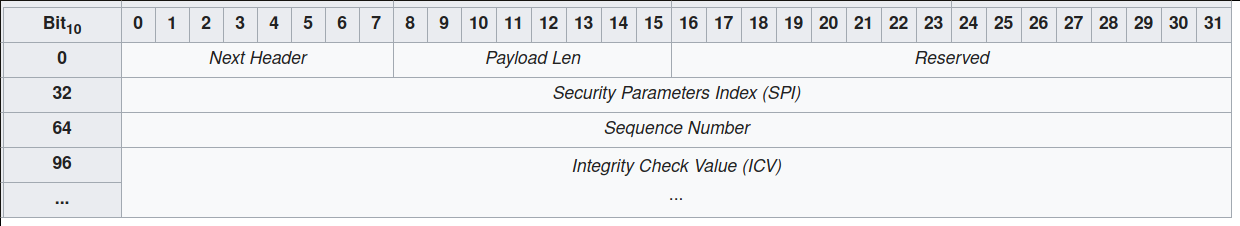
\includegraphics[width=\textwidth]{images/ah.png}
    \caption{The Authentication header}
\end{figure}

At the bottom there is a variable number of octets for authentication data.
This takes the HMAC of the immutable fields in the IP header.

The idea of immutable fields refers to the values in the header that cannot
change. These include the SPI, the sequence number, etc.

You may notice there is no explicit definition of mode whether it's tunnel
or transport. The mode is determined by the first parameter which was the type
of the next header.

\subsection{Encapsulating Security Payload (ESP)}
The Encapsulating Security Payload provides source authentication and data
integrity. It makes use of the same 32-bit counter as AH but it provides
data confidentiality using symmetric keys.

The ESP header is placed in the same place as the AH header. But now there
is also an ESP trailer and ESP Authentication. There are both placed at the
end of the packet in the respective order.

The ESP trailer is there to ensure the symmetric cipher has enough padding
to work.

\begin{figure}[h]
    \centering
    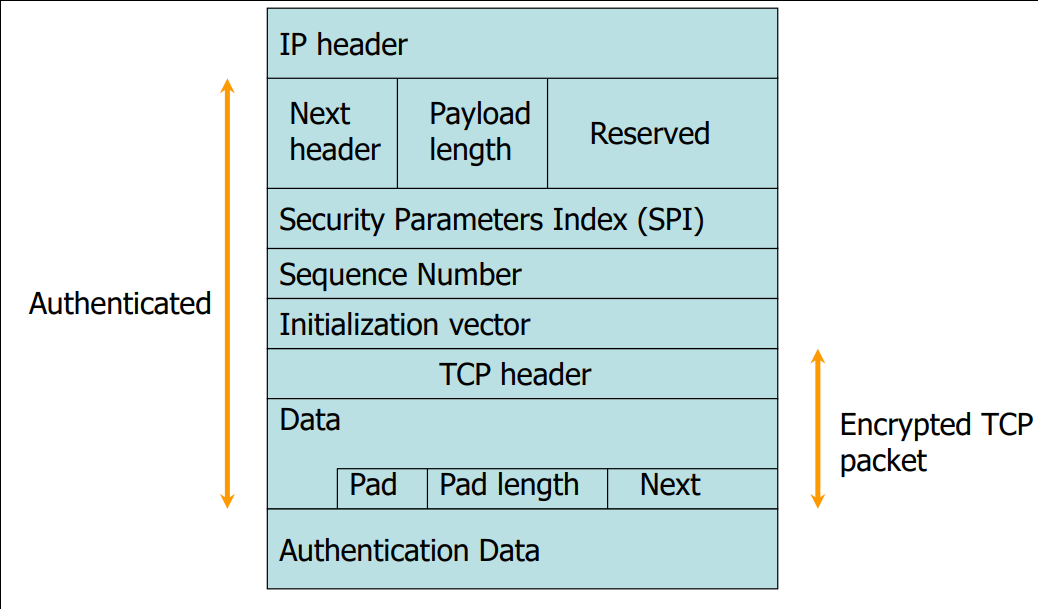
\includegraphics[width=\textwidth]{images/esppacket.png}
    \caption{The ESP header}
\end{figure}

Note that in tunnel mode the new IP address is not authenticated.
ESP is often used to implement VPNs.

\subsection{Security Authentication (SA)}
Security Authentications are asymmetric (uni-directional).
Thus you need an SA for inbound traffic and an SA for outbound.

All this information is stored in a \textbf{Security Association Database (SAD)}.
This along with a \textbf{Security Policy Database (SPD)} allows the computer
to correctly handle IPsec packets.

The SPD is two steps removed from the actual processing.
Imagine we're using the SPD for outgoing packets
(though inbound is also possible), to decide what SAD entries should be used,
and the SAD entries in turn describe the actual processing (SAD contains
the SPI).

You will notice that the SPD contains a lot of information from the SAD entry
this is okay in the case that there is not suitable entry in the SAD.
In this case we use the SPD to create a SAD entry.

\begin{figure}[h]
    \centering
    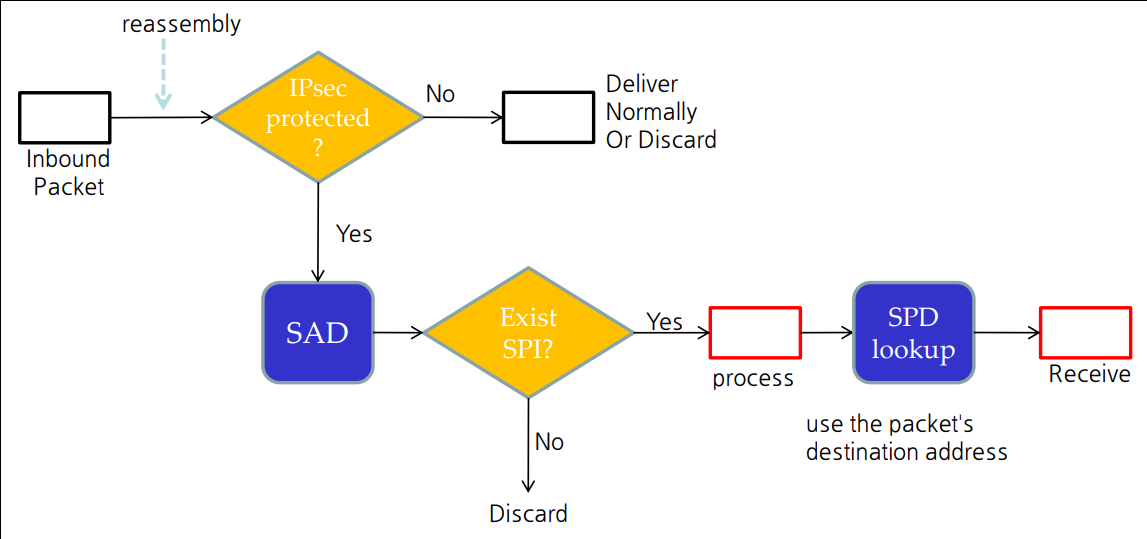
\includegraphics[width=\textwidth]{images/inboundprocess.png}
    \caption{The inbound process}
\end{figure}
\begin{figure}[h]
    \centering
    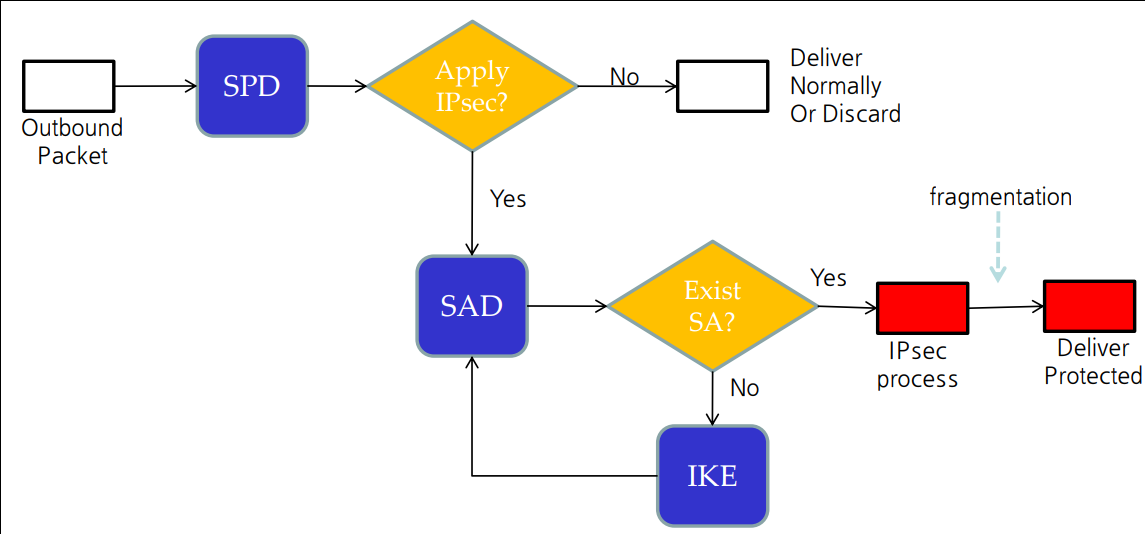
\includegraphics[width=\textwidth]{images/outboundprocess.png}
    \caption{The outbound process}
\end{figure}

\section{Intrusion Detection Systems (IDS) and family}
An intrusion is a set of actions that attempt to compromise the CIA triad
of computing resources via causing DoS, backdoors, planting viruses or
exploiting viruses.

We assume that it is possible to monitor activity of programs and users.
From this we come up with 3 simple steps,
\begin{enumerate}
    \item Monitoring and analysing host/network
    \item Identifying misuse/abnormal activities
    \item Assessing severity and raising alarms
\end{enumerate}

A good IDS needs high detection rate with low false alarms and minimum
overhead.

We can classify IDSs as either misuse detection and anomaly detection.

We can gather data via: Host based detection (command log and system calls),
Network based detection (packet headers and general traffic),
or both.

\textbf{Misuse detection}
is identifying the patterns of well known attacks to identify
intrusion. From this we also record the intrusions that occur to learn from
them. The problem here is that we struggle to detect new attacks.

\textbf{Anomaly detection}
is the opposite. Instead we search for deviation from normal usage to identify
intrusions. We must first establish what is normal behaviour and then report
deviations. This has the issue of high false positive rates since a new action
may be benign.

\textbf{Host-based Intrusion Detection System (HIDS)} is OS dependent and is
installed inside the host which means it is also possible to attack.

\textbf{Network Intrusion Detection System (NIDS)} is based on the packet
capturing of the network.

Another method of detection is \textbf{Support Vector Machines (SVN)-IDS}s.
This is pattern matching and categorising much like what we see in data science
and machine learning.

\textbf{Cooperative IDS}s use collective info from others to make instrusion
detection more accurate.

\subsection{SNORT}
SNORT is a NIDS system and is the most widely used one in the world. It can
even analyse streams, not just single packets.

SNORT first takes a packet and decodes it, then pre-processes it then runs it
through a detection engine. If it's part of the rules of logging it is then
logged and checked in the alerting system.

SNORT is a \textbf{signature based IDS}
thus they implement two phases of detection.
Phase 1 involves pattern matching. In Phase 2 we detect more complex patterns
based on what type of packet is actually being send, SNORT support 36 such
rules.

\subsection{Intrusion Prevention Systems (IPS)}
IPS is commonly an extension of intrusion detection. Since an IDS device is
passive we would like something more active.

This is more preferable since network attacks can happen fast and usually
only needs a small window of time to complete an attack.

Should be noted that though and IDS is cheap, IPS is \emph{very} expensive.

\subsection{Security Information Event management (SIEM)}
Many large organisations receive an insane number of alerts many of which are
false alarms. We have a few ways to solve this:
alert clustering which groups alerts together in meaningful ways,
only alerting if we match a predefined attack scenario (matching predefined
attack scenarios) or
we could also check if the attack could be successful in our system
and if so what would the outcome be (prerequisites/consequences).

SIEMs attempt to use all these techniques to help with false alarms.
A SIEM takes the logs and events and aggregates them (normalising and
analysing). For example, taking from networks, systems, applications etc.
We create a higher alarm if we find several related events happening.
This gives us a higher chance that we've detected an attack.

\section{Honeypots}
These are decoy systems designed to lure potential attackers away from
critical systems, collect information about the attackers activity
and encourages the attacker to stay on the system long enough for
admins to respond.

\end{document}

Filled with fabricated information that a legitimate user of the system
wouldn't be able to access. Once the hackers are within the network, admin
can observe behaviour.
